\chapter{Beschreibung ausgewählter Implementierungsdetails}
\label{chap:probleme}
In diesem Abschnitt der Arbeit werden die ausgewählten Systeme hinsichtlich ihrer technischen Umsetzung mit dem Rails-Framework untersucht. Bei der Betrachtung wird auf folgende Aspekte eingegangen:

\begin{enumerate}
\item Wartbarkeit der Erweiterungen
\item Nutzeroberfläche
\end{enumerate}


\section{Erweiterungen}
\label{dryverstoss}
Innerhalb des Rails Frameworks ist die Verwendung von Generatoren ein häufiges Mittel zur schnellen Entwicklung von funktionsfähigem Code (siehe Kapitel \ref{sec:railsgeneratoren} ). Drei der vier hier vorgestellten Systeme\footnote{Locomotive CMS benötigt durch die Verwendung von MongoDB und der Möglichkeit, individuelle Inhaltselemente im Backend zu erstellen keine installierbaren Erweiterungsmodule} bedienen sich zur Realisierung neuer Inhaltslemente ebenfalls eines Generatorskripts, der ein für das jeweilige CMS funktionsbereites Grundgerüst erzeugt. Exemplarisch soll hier das Ergebnis eines Generatoraufrufes in Refinery CMS aufgezeigt werden (Abb. \ref{sec.refineryoutput} ). Das erstellte Inhaltselement Projekt verfügt dabei über die Felder Titel und Beschreibung:


%\lstinputlisting[numbers=none, caption=Aufruf des Refinery Engine Generators mit Ausgabe des erzeugten Codegerüsts, label=refinerygenerator]{code/generator_refinery.rb}

\begin{lstlisting}[label=sec.refineryoutput,caption=Aufruf des Refinery Engine Generators mit Ausgabe des erzeugten Codegerüsts]
rails generate refinery_engineproject name:string description:text
create  vendor/engines/projects/app/controllers/admin/projects_controller.rb
create  vendor/engines/projects/app/controllers/projects_controller.rb
create  vendor/engines/projects/app/models/project.rb
create  vendor/engines/projects/app/views/admin/projects/_actions.html.erb
create  vendor/engines/projects/app/views/admin/projects/_form.html.erb
create  vendor/engines/projects/app/views/admin/projects/_projects.html.erb
create  vendor/engines/projects/app/views/admin/projects/_records.html.erb
create  vendor/engines/projects/app/views/admin/projects/_project.html.erb
create  vendor/engines/projects/app/views/admin/projects/_sortable_list.html.erb
create  vendor/engines/projects/app/views/admin/projects/edit.html.erb
create  vendor/engines/projects/app/views/admin/projects/index.html.erb
create  vendor/engines/projects/app/views/admin/projects/new.html.erb
create  vendor/engines/projects/app/views/projects/index.html.erb
create  vendor/engines/projects/app/views/projects/show.html.erb
create  vendor/engines/projects/config/locales/en.yml
create  vendor/engines/projects/config/locales/fr.yml
create  vendor/engines/projects/config/locales/lolcat.yml
create  vendor/engines/projects/config/locales/nb.yml
create  vendor/engines/projects/config/locales/nl.yml
create  vendor/engines/projects/config/routes.rb
create  vendor/engines/projects/db/migrate/create_projects.rb
create  vendor/engines/projects/db/seeds/projects.rb
create  vendor/engines/projects/features/manage_projects.feature
create  vendor/engines/projects/features/step_definitions/project_steps.rb
create  vendor/engines/projects/features/support/paths.rb
create  vendor/engines/projects/lib/generators/refinerycms_projects_generator.rb
create  vendor/engines/projects/lib/refinerycms-projects.rb
create  vendor/engines/projects/lib/tasks/projects.rake
create  vendor/engines/projects/readme.md
create  vendor/engines/projects/refinerycms-projects.gemspec
create  vendor/engines/projects/spec/models/project_spec.rb
\end{lstlisting}


Die durch den Aufruf erzeugten Dateien erfüllen dabei folgende wesentliche Funktionen:

\begin{description}
\item[Zeile 1]
Aufruf des Generatorbefehls
\item[Zeile 2-3]
Der Generator erzeugt zwei Rails-Controller zur Steuerung der Logik im Frontend und Backend des Content Managment Systems.
\item[Zeile 5-15]
Automatische Generierung von HTML-Views zur Darstellung aller im Frontend und Backend benötigten Komponenten. U.a. werden ein HTML-Formular zum Anlegen neuer Projekte im Backend (Zeile 6 \emph{\_form.html.erb}) und eine Auflistung von zur Verfügung stehenden Aktionen im Backend erstellt (Zeile 5 \emph{\_actions.html.erb})
\item[Zeile 4 und 22]
Erstellung des in Rails benötigten Models Project (Zeile 4 \emph{project.rb}) und der zur Speicherung in der Datenbank benötigten Migration (Zeile 22 \emph{create\_projects.rb})
\item[Zeile 21]
Erstellung einer Routing-Datei, welche die für das Frontend und Backend benötigten URL's bzw. Routen in der Rails-Anwendung registriert.
\item[Zeile 16-20]
Erstellung der für die Unterstützung von Mehrsprachigkeit notwendigen Konfigurationsdateien im YAML-
\item[Zeile 24-32]
Erzeugung der benötigten Dateien zur Unterstützung der Entwicklung von Tests sowie der Registrierung der Engine innerhalb der Rails-Anwendung (Zeile 28)
\end{description}

Bei Bedarf an weiteren Inhaltselementen ergibt sich schnell die Erkenntnis, das die Realisierung der Inhaltselemente mit Hilfe eines Generators redundanten Rails-Code erzeugt. Damit verstößt diese Art der Erweiterungsentwicklung gegen den in Rails propagierten Ansatz des DRY (Don't repeat yourself).

Diese Aussage soll im folgenden näher spezifiziert werden:


\begin{enumerate}
\item
Jedes Inhaltselement besitzt seine eigene Darstellungsrepräsentierung in Form von HTML-Views. Änderungen am Backend-Design des WCMS erfordern so eine Anpassung sämlicher verwendeter Erweiterungen. Die Erweiterung und das WCMS werden so sehr stark von einander abhängig.
\item
Werden Änderungen am Quellcode des WCMS vorgenommen (z.B. der Generatorskript erzeugt neuen HTML-Markup in den einzelnen Views), bedeutet dies für die Entwickler der Plugins ebenfalls eine Anpassung des Plugins\footnote{Diese Aussage bezieht sich auf geringfügige Änderungen}.
\item
Jedes Inhaltselement wird in einer eigenständigen Datenbanktabelle gespeichert. Ein Inhaltselement Projekt
benötigt so z.B. die Datenbanktabelle Projekt mit den Tabellenfeldern Name und Beschreibung. Bei häufiger Verwendung zusätzlicher Inhaltselemente entsteht somit schnell eine beachtliche Anzahl an zusätzlichen Tabellen\footnote{Die Zahl der Datenbanktabellen kann in Rails mit Hilfe von Single Table Inheritance (STI) minimiert werden.}.
\item
Die für die Inhaltselemente benötigten Datenbankschemas müssen in Form von in Rails üblichen Migrationen verwaltet werden. Dies erfordert einen entsprechenden Mehraufwand bei der Pflege der Erweiterungen.
\item
Jedes Plugin bestimmt durch die Bereitstellung seiner eigenen HTML-Views die Integration und das Aussehen der Erweiterung im Backend des WCMS. Ein einheitliches Erscheinungsbild aller Plugins ist somit nur schwer umsetzbar.
\item
Ein Import und Export von Inhaltselementen in das WCMS ist nur möglich, wenn die notwendigen Datenbanktabellen zuvor erzeugt wurden.
\item
Inhaltselemente müssen für ihre Erreichbarkeit im Frontend und Backend des WCMS im Routing der Rails-Anwendung registriert werden. Bei der Nutzung vieler Erweiterungen entstehen so zahlreiche zusätzliche Routingeinträge.
\item
Durch die Installation/Verwendung der umfassenden Erweiterungen wird die Gesamtgröße der Rails-Anwendung unnötig vergrößert (geringfügige Bedeutung).
\item
Durch das Laden zusätzlicher Rails-Controller und Models benötigt die Rails-Anwendung zusätzlichen Arbeitsspeicher und weist einen verlängerten Boot-Prozess auf (geringfügige Bedeutung).
\item
Durch das Laden zusätzlicher Rails-Controller und Models benötigt die Rails-Anwendung zusätzlichen Arbeitsspeicher und weist einen verlängerten Boot-Prozess auf (geringfügige Bedeutung).
\end{enumerate}


Der Verstoss gegen das Dry-Prinzip wird vor allem bei der Umsetzung der einzelnen Erweiterungs-Controller innerhalb von Refinery CMS ersichtlich. Dort wird mit Hilfe der im Controller verfügbaren Klassenmethode \emph{crudify} das gesamte Grundgerüst des Controllers dynamisch erzeugt\footnote{Die Methode \emph{crudify} erstellt mit Hilfe von Ruby-Metaprogrammierung die gesamte Logik des Controllers. Alle Aktionen, die der Controller verwaltet, werden so erst zur Laufzeit der Rails-Anwendung generiert. Nähere Informationen zu \emph{Crudify} im Anhang der Arbeit unter Abschnitt \ref{crudifyanhang}.}. Die Methode kann dabei verschiedene Parameter aufnehmen, an Hand deren die Ausgabe gesteuert werden kann. Alle neu erzeugten Inhaltselemente sind in ihrer Grundstruktur als Rest-basierte Ressourcen anzusehen, die mit Hilfe eines angepassten Rails-Generators in das jeweilige Backend des WCMS eingebunden werden. Durch diese gegenseitigen Abhängigkeiten ist die Wartbarkeit der Erweiterungen sehr von der Entwicklung des Kernsystems abhängig. Vorallem Änderungen am Generatorskript des jeweiligen WCMS ziehen häufig Anpassungen bei den erzeugten Plugins nach sich. Durch die Reduzierung der Abhängigkeiten zwischen WCMS und Erweiterung (vor allem auf Darstellungsebene durch die verwendeten Views) kann eine stabilere Entwicklungsbasis geliefert werden.

\lstinputlisting[language=Ruby, caption=Projects-Controller mit verwendeter crudify-Methode und optionalen Parametern]{code/crudify_controller.rb}


\section{Nutzeroberfläche}

Die Nutzeroberflächen der vorgestellten Web Content Management Systemen sind durch die Kombination individueller HTML, CSS und JavaScript-Dateien zusammengestellt wurden. Bei der Nutzung der Systeme und der Durchführung von Erweiterungsentwicklungen ergeben sich somit folgende Eindrücke:

\begin{enumerate}
\item
Das Backend der Systeme wird in Rails mit Hilfe verschiedener HTML-Views und Partials (wiederverwendbare HTML-Views) erzeugt. Dies resultiert in einer verstärkten Antwortzeit\footnote{Die Antwortzeit (response time) ist die Zeitdauer, die eine Anwendung bzw. ein System benötigt, um eine Anfrage von außen zu verarbeiten (z.B. UI-Aktion) \citep[S. 21] {FowlerPatterns}.}, da das Rails-Framework die gesamte Backend-Oberfläche erst neu erzeugen muss. Vor allem bei der Nutzung von Browser CMS und Refinery CMS macht sich die Art der Backend-Generierung bemerkbar.
\item
Die Nutzeroberfläche der Medienverwaltung (Bilder und Dateien) erlaubt nur eine Auflistung aller im System vorhandenen Ressourcen (Abb. \ref{medeinverwaltungliste}). Bei größeren Datenmengen kommt diese Art der Darstellung schnell an ihre Leistungsgrenzen. Diese Beschränkung der Nutzeroberfläche besteht bei allen untersuchten WCMS.
\item
Das verwendete JavaScript zur Realisierung von Dialogen (z.B. Auswahl eines Bildes) und Backend-Funktionalitäten (z.B. Einbindung eines WYSIWYG-Editors) wird in Form einfacher JavaScript-Funktionen in das von Rails erzeugte Template eingebunden (Abb. /ref{refineryimagedialog}). Die Skripte sind dabei nicht modular aufgebaut und machen so eine Integration individueller Funktionalitäten nur schwer möglich.
\end{enumerate}

\begin{figure}[!H]
\begin{center}
\label{medeinverwaltungliste}
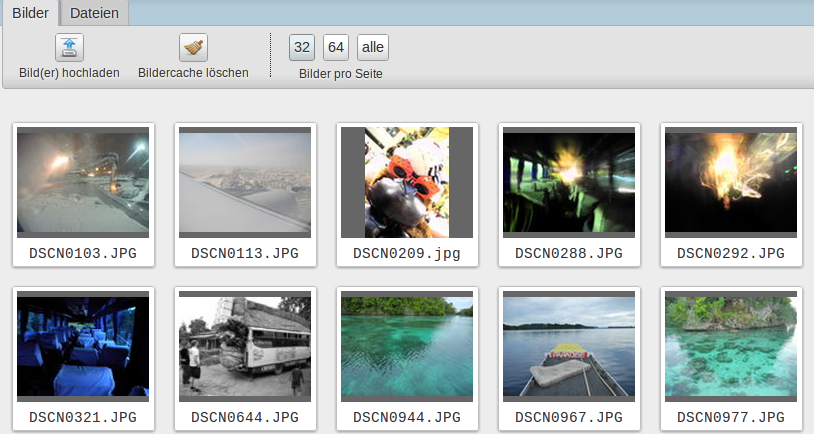
\includegraphics[scale=0.5]{images/analyse/alchemy/ressourcen.png}
\caption{Ressourcen-Auflistung ohne Möglichkeiten der Strukturierung in Alchemy CMS. Für die anderen Systeme ergibt sich ein ähnliches Gesamtbild.}
\end{center}
\end{figure}

\begin{lstlisting}[label=refineryoutput,caption=Beispiel für eine JavaScript-Funktion zur Realisierung des Bildauswahldialogs in Refinery CMS. Das Codebeispiel zeigt ebenfalls die Abhängigkeit zu dem verwendeten HTML-Markup (z.B. Zeile 18)]

var image_dialog = {
  initialised: false
  , callback: null
  , init: function(callback){
    if (!this.initialised) {
      this.callback = callback;
      this.init_tabs();
      this.init_select();
      this.init_actions();
      this.initialised = true;
    }
    return this;
  }
  //...
  , set_image: function(img){
    if ($(img).length > 0) {
      $('#existing_image_area_content ul li.selected').removeClass('selected');
      $(img).parent().addClass('selected');
      var imageId = $(img).attr('data-id');
      var geometry = $('#existing_image_size_area li.selected a').attr('data-geometry');
      var size = $('#existing_image_size_area li.selected a').attr('data-size');
      var resize = $("#wants_to_resize_image").is(':checked');
      image_url = resize ? $(img).attr('data-' + size) : $(img).attr('data-original');
      //...
    }
  }
  //...
};
\end{lstlisting}

